% Options for packages loaded elsewhere
\PassOptionsToPackage{unicode}{hyperref}
\PassOptionsToPackage{hyphens}{url}
\PassOptionsToPackage{dvipsnames,svgnames,x11names}{xcolor}
%
\documentclass[
  12pt]{article}

\usepackage{amsmath,amssymb}
\usepackage{setspace}
\usepackage{iftex}
\ifPDFTeX
  \usepackage[T1]{fontenc}
  \usepackage[utf8]{inputenc}
  \usepackage{textcomp} % provide euro and other symbols
\else % if luatex or xetex
  \usepackage{unicode-math}
  \defaultfontfeatures{Scale=MatchLowercase}
  \defaultfontfeatures[\rmfamily]{Ligatures=TeX,Scale=1}
\fi
\usepackage{lmodern}
\ifPDFTeX\else  
    % xetex/luatex font selection
\fi
% Use upquote if available, for straight quotes in verbatim environments
\IfFileExists{upquote.sty}{\usepackage{upquote}}{}
\IfFileExists{microtype.sty}{% use microtype if available
  \usepackage[]{microtype}
  \UseMicrotypeSet[protrusion]{basicmath} % disable protrusion for tt fonts
}{}
\makeatletter
\@ifundefined{KOMAClassName}{% if non-KOMA class
  \IfFileExists{parskip.sty}{%
    \usepackage{parskip}
  }{% else
    \setlength{\parindent}{0pt}
    \setlength{\parskip}{6pt plus 2pt minus 1pt}}
}{% if KOMA class
  \KOMAoptions{parskip=half}}
\makeatother
\usepackage{xcolor}
\setlength{\emergencystretch}{3em} % prevent overfull lines
\setcounter{secnumdepth}{5}
% Make \paragraph and \subparagraph free-standing
\ifx\paragraph\undefined\else
  \let\oldparagraph\paragraph
  \renewcommand{\paragraph}[1]{\oldparagraph{#1}\mbox{}}
\fi
\ifx\subparagraph\undefined\else
  \let\oldsubparagraph\subparagraph
  \renewcommand{\subparagraph}[1]{\oldsubparagraph{#1}\mbox{}}
\fi


\providecommand{\tightlist}{%
  \setlength{\itemsep}{0pt}\setlength{\parskip}{0pt}}\usepackage{longtable,booktabs,array}
\usepackage{calc} % for calculating minipage widths
% Correct order of tables after \paragraph or \subparagraph
\usepackage{etoolbox}
\makeatletter
\patchcmd\longtable{\par}{\if@noskipsec\mbox{}\fi\par}{}{}
\makeatother
% Allow footnotes in longtable head/foot
\IfFileExists{footnotehyper.sty}{\usepackage{footnotehyper}}{\usepackage{footnote}}
\makesavenoteenv{longtable}
\usepackage{graphicx}
\makeatletter
\def\maxwidth{\ifdim\Gin@nat@width>\linewidth\linewidth\else\Gin@nat@width\fi}
\def\maxheight{\ifdim\Gin@nat@height>\textheight\textheight\else\Gin@nat@height\fi}
\makeatother
% Scale images if necessary, so that they will not overflow the page
% margins by default, and it is still possible to overwrite the defaults
% using explicit options in \includegraphics[width, height, ...]{}
\setkeys{Gin}{width=\maxwidth,height=\maxheight,keepaspectratio}
% Set default figure placement to htbp
\makeatletter
\def\fps@figure{htbp}
\makeatother

\addtolength{\oddsidemargin}{-.5in}%
\addtolength{\evensidemargin}{-1in}%
\addtolength{\textwidth}{1in}%
\addtolength{\textheight}{1.7in}%
\addtolength{\topmargin}{-1in}%
\makeatletter
\@ifpackageloaded{caption}{}{\usepackage{caption}}
\AtBeginDocument{%
\ifdefined\contentsname
  \renewcommand*\contentsname{Table of contents}
\else
  \newcommand\contentsname{Table of contents}
\fi
\ifdefined\listfigurename
  \renewcommand*\listfigurename{List of Figures}
\else
  \newcommand\listfigurename{List of Figures}
\fi
\ifdefined\listtablename
  \renewcommand*\listtablename{List of Tables}
\else
  \newcommand\listtablename{List of Tables}
\fi
\ifdefined\figurename
  \renewcommand*\figurename{Figure}
\else
  \newcommand\figurename{Figure}
\fi
\ifdefined\tablename
  \renewcommand*\tablename{Table}
\else
  \newcommand\tablename{Table}
\fi
}
\@ifpackageloaded{float}{}{\usepackage{float}}
\floatstyle{ruled}
\@ifundefined{c@chapter}{\newfloat{codelisting}{h}{lop}}{\newfloat{codelisting}{h}{lop}[chapter]}
\floatname{codelisting}{Listing}
\newcommand*\listoflistings{\listof{codelisting}{List of Listings}}
\makeatother
\makeatletter
\makeatother
\makeatletter
\@ifpackageloaded{caption}{}{\usepackage{caption}}
\@ifpackageloaded{subcaption}{}{\usepackage{subcaption}}
\makeatother
\ifLuaTeX
  \usepackage{selnolig}  % disable illegal ligatures
\fi
\usepackage[]{natbib}
\bibliographystyle{agsm}
\usepackage{bookmark}

\IfFileExists{xurl.sty}{\usepackage{xurl}}{} % add URL line breaks if available
\urlstyle{same} % disable monospaced font for URLs
\hypersetup{
  pdftitle={Assessing the Impact of Outliers on Least Square Variogram Model},
  pdfauthor={Caterina Daidone, Marco Zanotti},
  pdfkeywords={spatial statistics, outliers, variogram},
  colorlinks=true,
  linkcolor={blue},
  filecolor={Maroon},
  citecolor={Blue},
  urlcolor={Blue},
  pdfcreator={LaTeX via pandoc}}


\begin{document}


\def\spacingset#1{\renewcommand{\baselinestretch}%
{#1}\small\normalsize} \spacingset{1}


%%%%%%%%%%%%%%%%%%%%%%%%%%%%%%%%%%%%%%%%%%%%%%%%%%%%%%%%%%%%%%%%%%%%%%%%%%%%%%

\date{February 28, 2024}
\title{\bf Assessing the Impact of Outliers on Least Square Variogram
Model}
\author{
Caterina Daidone, Marco Zanotti\\
University of Milano Bicocca\\
}
\maketitle

\bigskip
\bigskip
\begin{abstract}
It is a matter of common experience that ore values often do not follow
the normal (or lognormal) distributions assumed for them, but, instead,
follow some other heavier-tailed distribution. This study reviews the
two most popular methods for the variogram estimation, that is the
classical and the robust variograms. Moreover, a simulation study is
performed to assess the impact of outliers on the variogram estimates.
It is shown that the use of the robust variogram yields stable estimates
when the scale of the contamination increases.
\end{abstract}

\noindent%
{\it Keywords:} spatial statistics, outliers, variogram
\vfill

\newpage
\spacingset{1.9} % DON'T change the spacing!

\setstretch{1.5}
\section{Introduction}\label{introduction}

an introductory section describing the main task tackled in the paper
(along with relevant bibliographic references)

\section{Methods}\label{methods}

a methodological section covering methods

\section{Simulation}\label{simulation}

In order to assess the impact of outliers on the variogram estimation
based on the classical and the robust approaches, a simulation study is
permformed. Simulating Gaussian Random Fields (GRF) and Contaminated
Gaussian Random Fields (CGRF) involves different approaches due to the
added complexity of contamination. GRFs solely need a mean and
covariance function. This function dictates the smoothness and spatial
dependence of the field. Common methods for generating GRF include the
spectral method (using Fast Fourier Transforms) and the Cholesky
decomposition. Simulating CGRF, instead, introduces an additional layer
of complexity. In this case, the underlying GRF represents the ``true''
signal, while the contamination acts as an independent noise process.
Common approaches involve generating the GRF first, then adding a
separate noise field with its own properties (e.g., mean, variance,
spatial dependence). Alternatively, one can directly simulate the CGRF
by incorporating the contamination into the covariance function itself.

Following \citet{cre:1980}, the departure from Gaussianity is obtained
simulating a GRF with probability \(1 - \epsilon\) and a CGRF with
probability \(\epsilon\).\\
\[
\begin{cases}
  N(0, \sigma^2), \;\;\;\;\;\;\; with \; probability \; 1-\epsilon \\
  N(0, k^2 \sigma^2), \;\;\;\; with \; probability \; \epsilon
\end{cases}
\]

where \(\epsilon\) is the probability of contamination and \(k\)
measures the scale of the contamination. To practically simulate the
underlying GRF, the grf function of the geoR package in R is used.

The simulation is based on 1000 spatial points on a regular grid, with a
mean of 0 and a covariance function with parameters \(\sigma^2 = 1\) and
\(\phi = 0.25\). The base scenario, that is no contamination, is
simulated with \(\epsilon = 0\).

\begin{center}
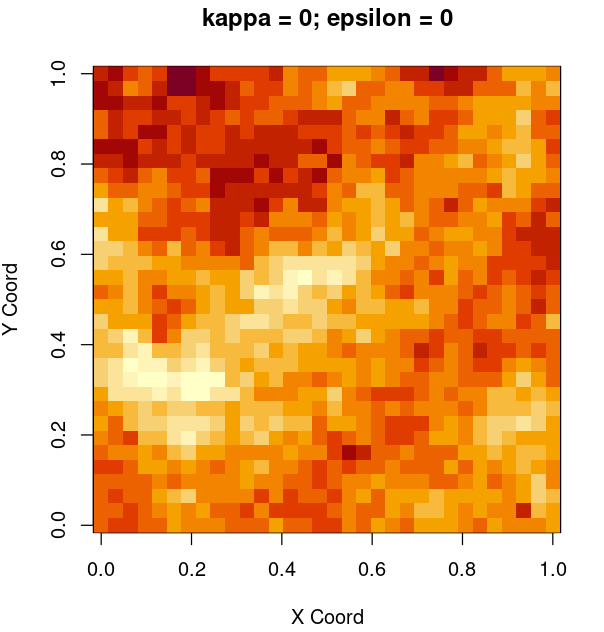
\includegraphics[width=3.125in,height=\textheight]{img/grf.png}
\end{center}

Then six different contaminated scenarios are simulated based on the
combinations of \(epsilon = (0.05, 0.1, 0.2)\) and \(kappa = (5, 10)\),
to assess the impact of contamination on the variogram estimation under
different circumstances.

\begin{center}
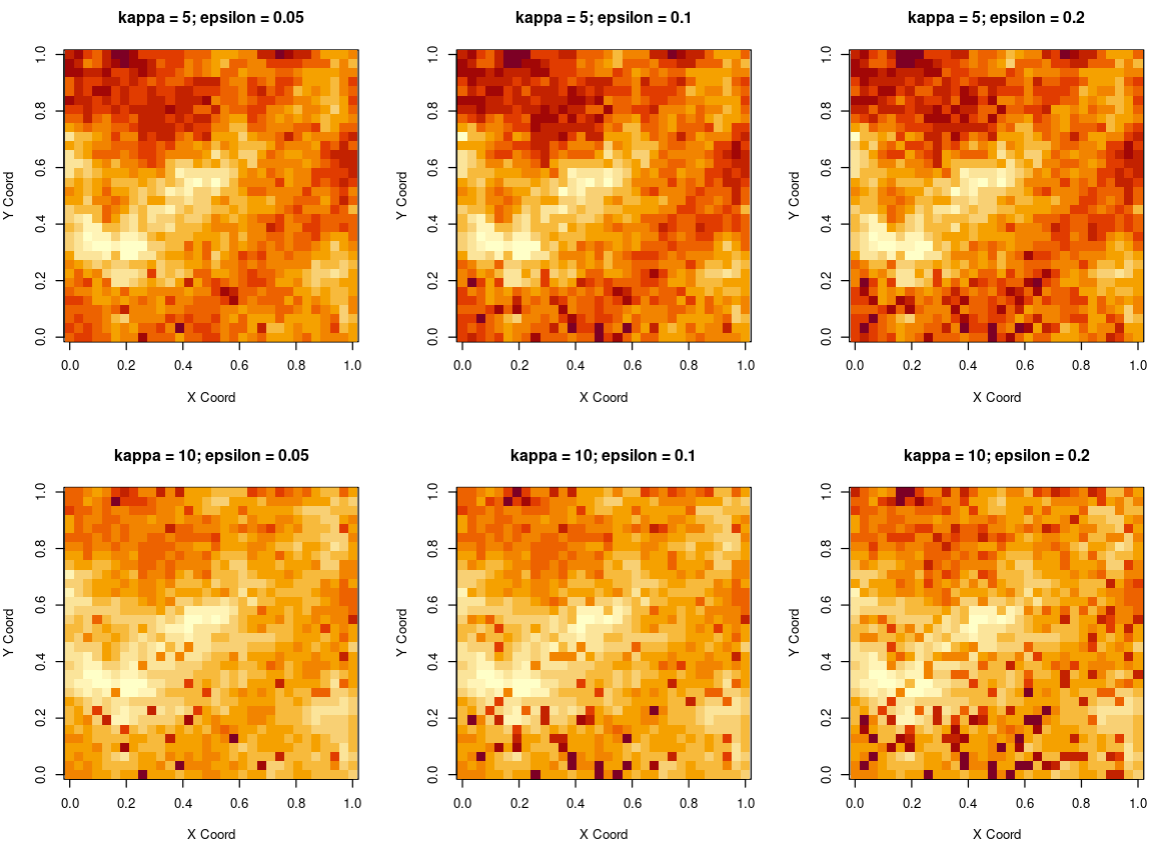
\includegraphics[width=5.20833in,height=\textheight]{img/cgrf.png}
\end{center}

Nugget and different levels of spatial correlation are not considered in
this simulation study but they can be easily added to the simulation
process.

\section{Results}\label{results}

The variogram estimation is performed using the classical (in black) and
the robust (in red) approaches. The two methods are compared on the
different simulated scenarios to assess their robustness to
contamination. Moreover, given that outliers are almost always
problematic for kriging, a variogram model is also estimated, using the
OLS estimator, to see how the outliers affect the model estimates. The
estimation process is performed using the functions variog and variofit
of the geoR package in R.

The base scenario, that is no contamination, shows that the two methods
provide almost identical results.

\begin{center}
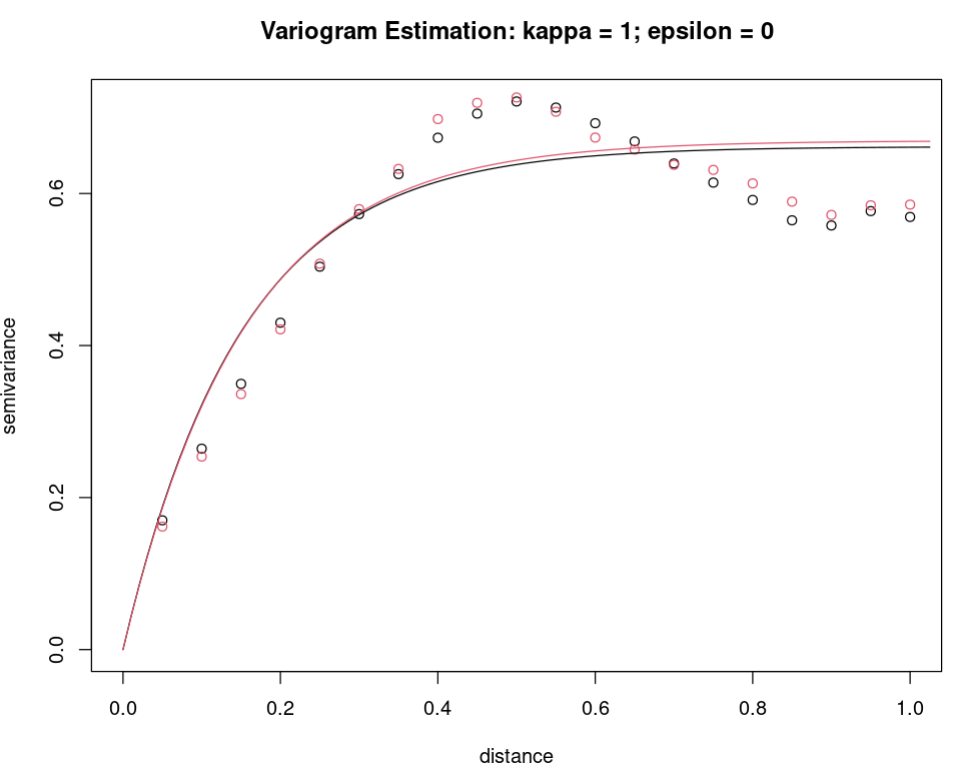
\includegraphics[width=5.20833in,height=\textheight]{img/variog_grf_ols.png}
\end{center}

In the presence of contamination, instead, the two methods provide
different results. If the results are analyzed in terms of the outliers'
scale (\(kappa\)), it is possible to observe two different behaviours.
For small outliers' scale, that is \(kappa = 5\), the two methods
provide similar estimations independently of the number of outliers
(\(\epsilon\)). However, for large outliers' scale, that is
\(kappa = 10\), the estimates are more different the higher the number
of outliers.

\begin{center}
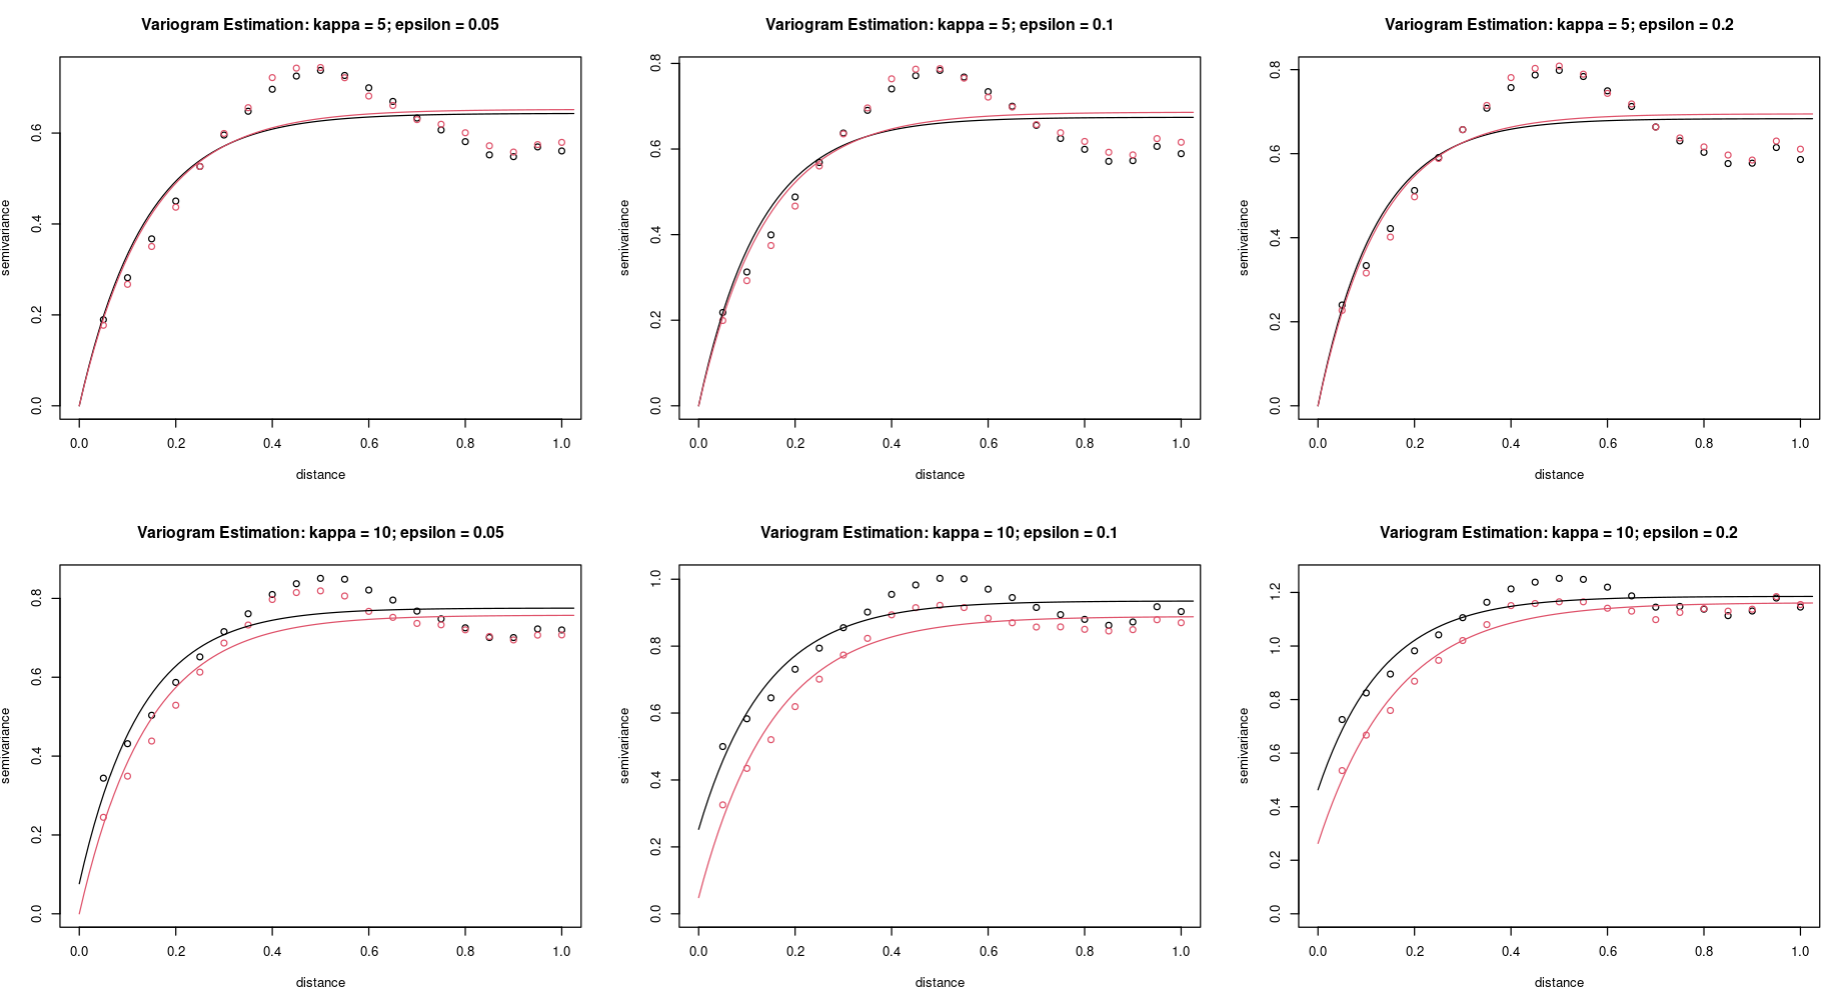
\includegraphics[width=6.25in,height=\textheight]{img/variog_cgrf_ols.png}
\end{center}

As expected, from theoretical considerations, the robust variogram
estimates are generally smaller than the classical ones. Indeed, the
classical approach is heavily influenced primarily by the scale of the
outliers, while the robust approach is less sensitive to the
contamination. Moreover, the scale of the contamination also strongly
affects the estimation of the nugget (which should be always 0), but the
robust approach is much less sensitive to this issue.

\begin{center}
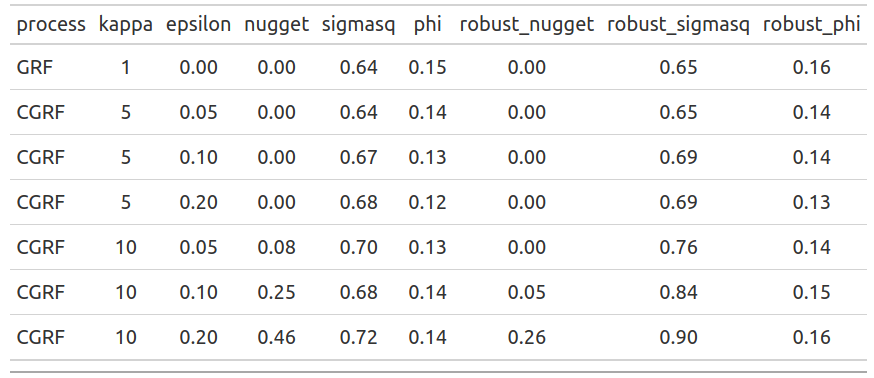
\includegraphics[width=5.20833in,height=\textheight]{img/variog_est_ols.png}
\end{center}

\section{Conclusion}\label{conclusion}

The theoretical considerations suggest that the robust variogram is less
sensitive to the presence of outliers. For this reason it should be
preferred when the data are contaminated. The simulation study confirms
this results and shows that the robust variogram yields stable estimates
when the scale of the contamination increases. However, if the scale of
the contamination is small, then the two methods provide similar
results.


  \bibliography{bibliography.bib}


\end{document}
